% This template has been downloaded from:
% http://www.latextemplates.com

% Original author:
% Ted Pavlic (http://www.tedpavlic.com)
%
% Modified by:
% Charles Newey (http://assemblyco.de)
%----------------------------------------

% Declare document
\documentclass[11pt]{article}

% Packages
\usepackage[superscript]{cite} % Superscript citations
\usepackage{fancyhdr} % Required for custom headers
\usepackage{lastpage} % Required to determine the last page for the footer
\usepackage{extramarks} % Required for headers and footers
\usepackage[usenames,dvipsnames]{color} % Custom colours
\usepackage{graphicx} % Images
\usepackage{tabularx} % Tables
\usepackage[colorlinks]{hyperref} % For URLs
\usepackage{lscape}

\hypersetup{ % Set up hyperref colours (http://stackoverflow.com/q/2770347)
	citecolor=Red
}
 
% Margins
\topmargin=0in
\evensidemargin=0in
\oddsidemargin=0in
\textwidth=6.5in
\textheight=8.0in
\headsep=0.25in
\linespread{0.9} % Line spacing

% Set up the header and footer
\pagestyle{fancy}
\lhead{Charles Callum Newey} % Top left header
\chead{} % Top center head
\rhead{CS25210 Assignment\firstxmark} % Top right header
\lfoot{\lastxmark} % Bottom left footer
\cfoot{} % Bottom center footer
\rfoot{Page\ \thepage\ of\ \protect\pageref{LastPage}} % Bottom right footer
\renewcommand\headrulewidth{0.4pt} % Size of the header rule
\renewcommand\footrulewidth{0.4pt} % Size of the footer rule

\setlength\parindent{0pt} % Removes all indentation from paragraphs
\renewcommand{\refname}{} % Removes bibliography title

% Title page
\title{
\vspace{2in}
\textmd{\textbf{CS25210 Assignment \\ Client-Side Graphics Programming for the Web}}\\
\normalsize\vspace{0.1in}\small{Due}\\
\vspace{0.1in}\large{\textit{22 April 2014}}
\vspace{3in}
}

\author{\textbf{Charles Callum Newey (ccn4)}}
\date{Word count: 1041}

% Make title page, ToC and other introductory elements
\begin{document}
\maketitle
\newpage
\tableofcontents
\newpage

% Begin the actual document
\begin{section}{Executive Summary}
    The game that I decided to develop is simple in nature, as I felt that a game need not be complex to be fun to play or visually pleasing. The game (called Zombie Pendemic - \textit{pun intended}) is a simple mouse-based shooter - the user plays as a ``turret'' in the centre of the canvas, battling against a never-ending onslaught of zombies. \\
    
    The player would have to ``shoot'' the zombies by clicking in the same direction. The player's score would increase when zombies were hit by bullets - with different score values for each ``type'' of zombie. The idea was for the game to get more difficult for the player over time. This was fairly straightforward when it came to implementation - the number of zombies on-screen simply increases as a function of the player's score. The zombies also increase in speed as the game progresses, ensuring that each game lasts for just enough time to stay interesting. Storyboards are included at the end of this document in the ``Appendices'' section (\ref{appendices}). \\
    
    One of the major design choices that I made early on in development was to make all of the sprites and sounds myself - this ensured that I had complete control of the look and feel of the game. This proved to be a lot more work than I had originally anticipated, but I am satisfied with the result.
\end{section}

\begin{section}{Technical Overview}
    \begin{subsection}{Technologies Used}
    		Obviously, the broad architectural choices for the game were pre-defined - that is, HTML5, CSS and JavaScript. However, web application development is complicated and involves more than just language and rendering choices. In keeping with my original desire to keep the project as original as possible, I have used no external programming libraries (aside from Google Analytics\cite{GAnalytics}), and nothing other than a font from Google's Font API\cite{GFonts}. This allowed me to have full control over the quality and performance of my code base. \\
    		
    		I dislike the idea of using a library such as JQuery or MooTools, as there are few advantages that I could see for this assignment. JQuery is particularly useful for manipulating the DOM and making AJAX calls (amongst other things), but in this instance, I didn't need either of those functionalities - the extra functionality would have been somewhat wasted.
    \end{subsection}
    
    \clearpage
    \begin{subsection}{Alternative Technologies}
    		There are a number of existing technologies that could serve in place of HTML5 and JavaScript, such as Flash or Silverlight - however, these are far less popular (and less common, to an extent) than HTML5 and JS. Flash and Silverlight require additional plugins, and are also proprietary technologies - meaning that support across browsers and operating systems is varied. This makes HTML5 and JS the most sensible (and modern) choice. \\
    		
    		There are also external libraries for JavaScript development (such as JQuery and MooTools), that make a lot of complex functions readily available - however, I have decided to forgo the use of these in favour of more control over performance and stability. \\
    		
    		I chose to make a slightly unusual architectural decision within the application. Most HTML5 canvas games repaint the entire canvas on each subsequent frame of the animation - this struck me as wasteful, as this involves a lot of unnecessary redrawing. My implementation, then uses three separate layered canvases to hold several UI elements that may overlap. In this case; one canvas to draw the health bar, one to draw the bullets, and another for the zombies and the main turret animation. This helps to minimise CPU overhead - at the expense of a small amount of memory.
    \end{subsection}
\end{section}
    
    \begin{section}{Testing}
    		The game has been tested as well as possible - on several operating systems using several browsers. This includes (but is not limited to) Firefox, Google Chrome, Chromium, Internet Explorer and Safari. It was also tested on various operating systems and mobile devices; Windows, Mac OS, Linux (various distributions, but mostly Arch Linux), iPads and Android devices. The only problems I encountered really were with the HTML5 audio API, which proved troublesome on some older Android devices. Aside from the audio issues, the game was perfectly playable (and still fun, at that) on an Android device. \\
    		
    		There was a particularly strange bug I encountered on the Linux x86 build of Firefox (running on Arch Linux) - Firefox's JS implementation would garbage-collect memory that was still in use by the main application, causing the game to freeze and crash. This hasn't happened in any other browser or operating system that I have tested, so as far as I could tell, this was an isolated case.\\
    		
    		I also found that the game had some trouble with freezing on some older iPad devices - I couldn't work out the cause of this easily, as the default browsers on iOS devices don't include developer tools. However, the game worked surprisingly well on a number of mobile devices, and responded just as well to tapping (in the case of touchscreens) as well as clicking.
    		
 		\vspace{0.5in}
		\begin{figure}[htp]
			\centering
			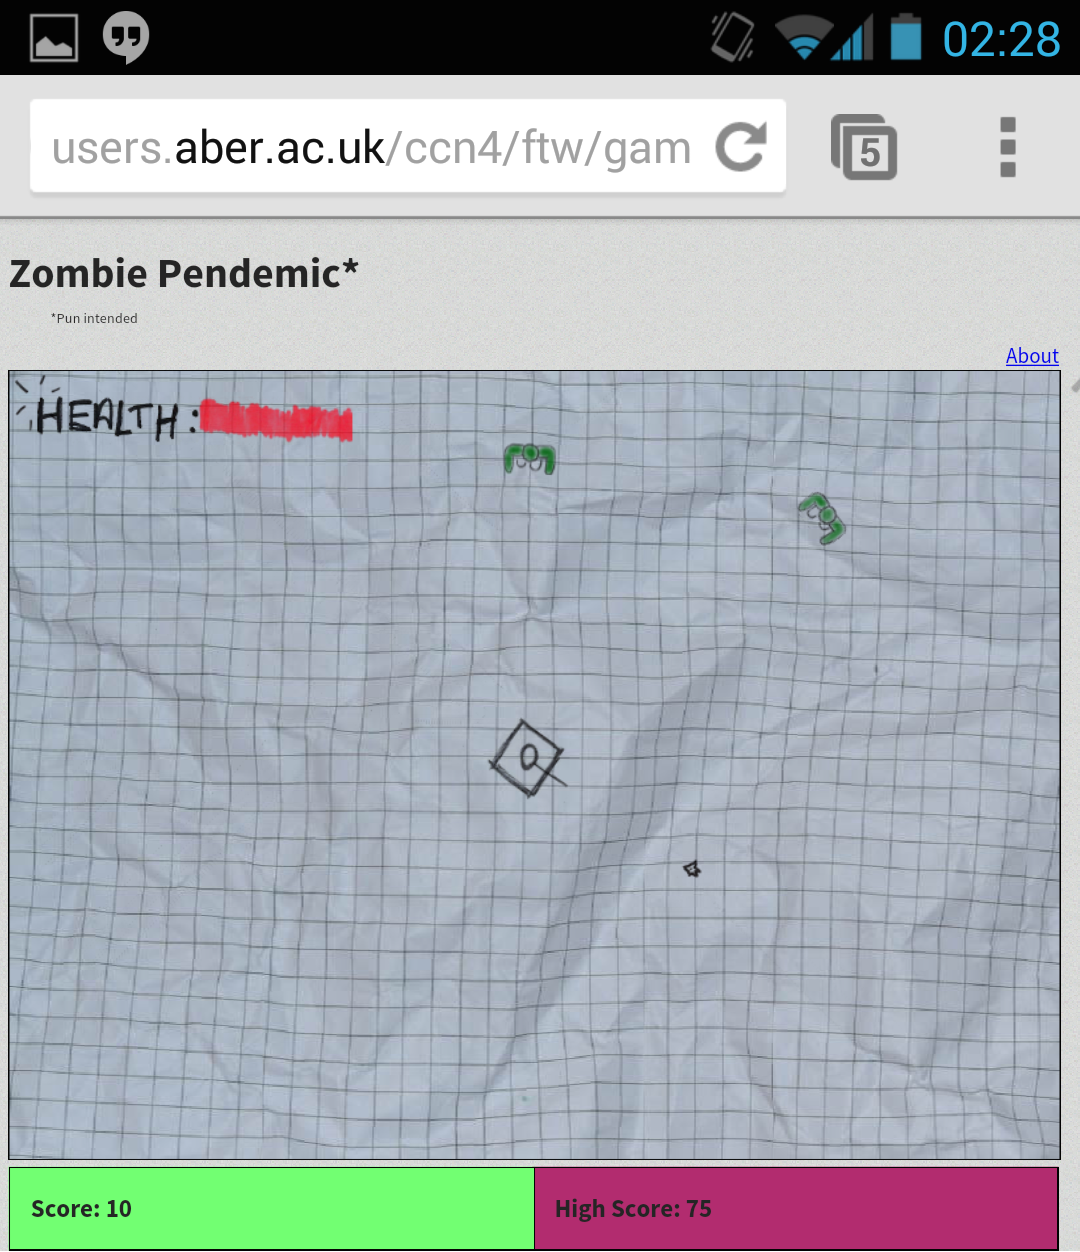
\includegraphics[height=0.5\columnwidth]{img/android}
			\caption{Gameplay on an Android device}
		\end{figure}
		
		\begin{figure}[htp]
			\centering
			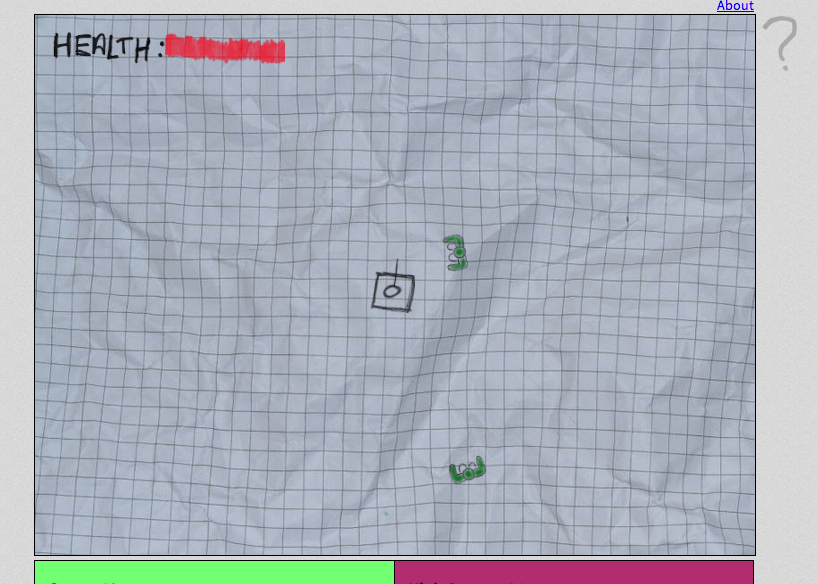
\includegraphics[height=0.6\columnwidth]{img/osx}
			\caption{Gameplay on Mac OS X (in Chrome)}
		\end{figure}
	\end{section}
    
\clearpage
\begin{section}{Reflections and Future Work}
    		If I were to repeat the project, I would have probably implemented a slightly more complex game. Although I am happy with the outcome, I would have liked to create something a little more challenging - both to make and to play. Also, I would have chosen a different style of game - one that was more conducive to keyboard control as the only keyboard interaction I could realistically fit in was pausing and resuming the game. \\
    		
    		One thing I would have added to this project (given more time), would potentially be some form of multiplayer functionality. This is possible (and in fact, quite simple) using JavaScript and WebSockets. WebSockets are an emerging web technology that is useful for full-duplex communications over open sockets in a web browser\cite{WebSockets}. This differs from AJAX as AJAX opens new connections upon every request. Because WebSockets have a greater longevity, they have a better latency (due to needing to open sockets far less frequently) - and this makes them far more suitable for a multiplayer online web game. \\
    		
    		Overall, I'm very happy with the decision to make all of the game sprites and sounds myself - I am happy with the drawn effect of the entire game - it's exactly the effect I wanted to achieve. Graphically, the game isn't ground-breaking - but I think it looks pleasant, and the game is definitely good fun to play.
\end{section}


% References
\nocite{LaTeXTemplate}

% Format bibliography/refs
\newpage
\begin{section}{References}
	\bibliographystyle{acm}
	\bibliography{References}
\end{section}

\clearpage
\begin{landscape}
    \begin{section}{Appendices}
    \label{appendices}
        \begin{subsection}{Storyboards}
        \vspace{0.5in}
            \begin{figure}[htp]
      		\centering
                    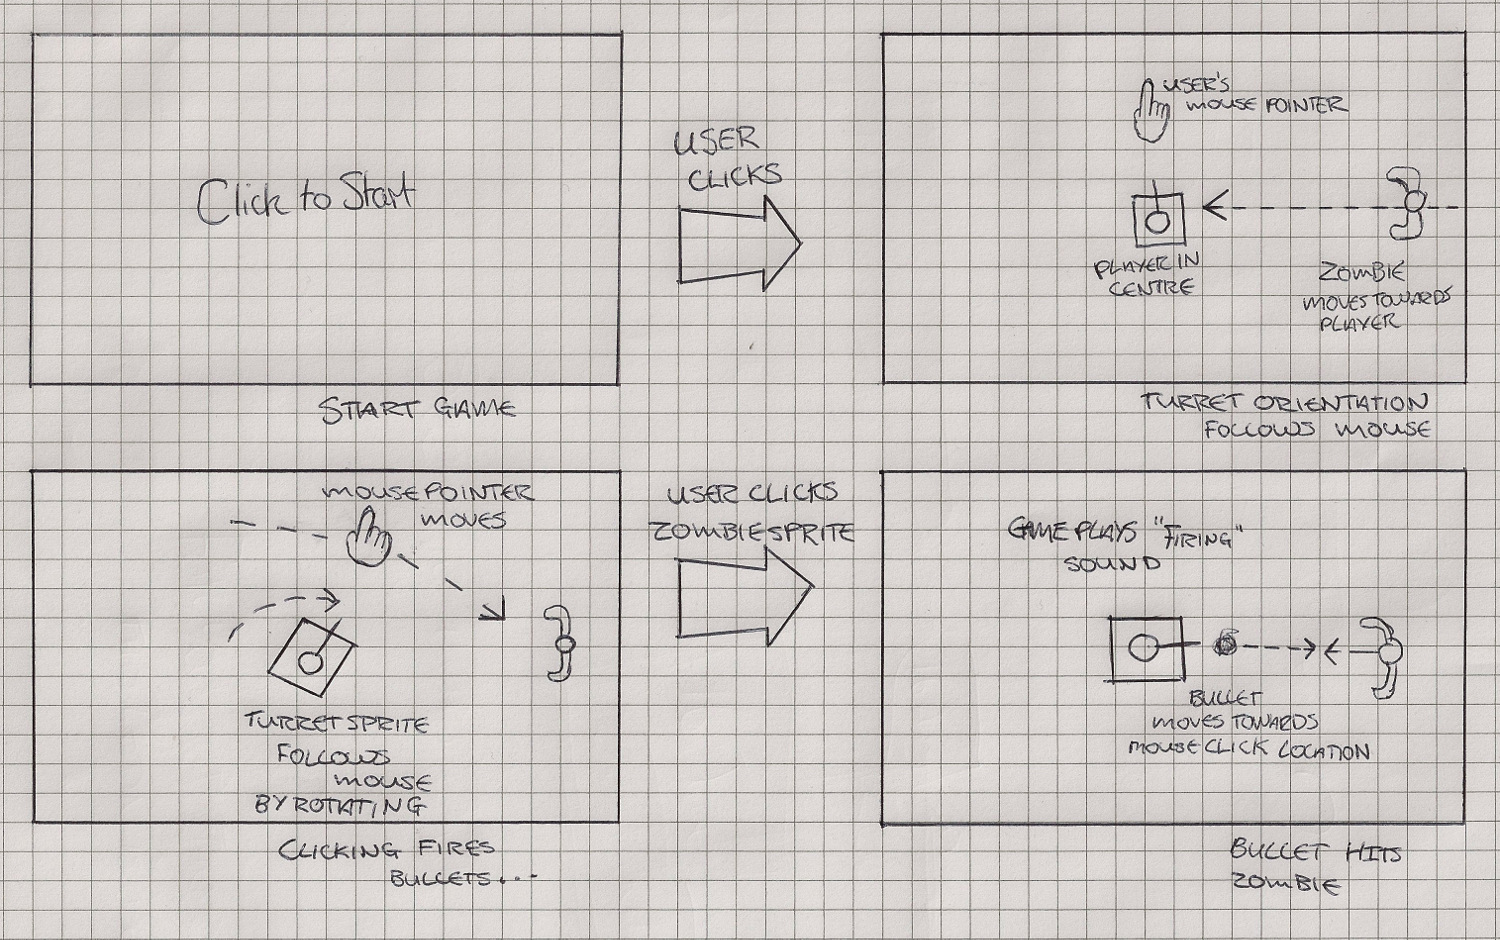
\includegraphics[height=0.5\columnwidth]{img/storyboard_1}
	    		\caption{First storyboard in sequence}
    		\end{figure}
    		
    		\clearpage
    		\begin{figure}[htp]
	    		\centering
                    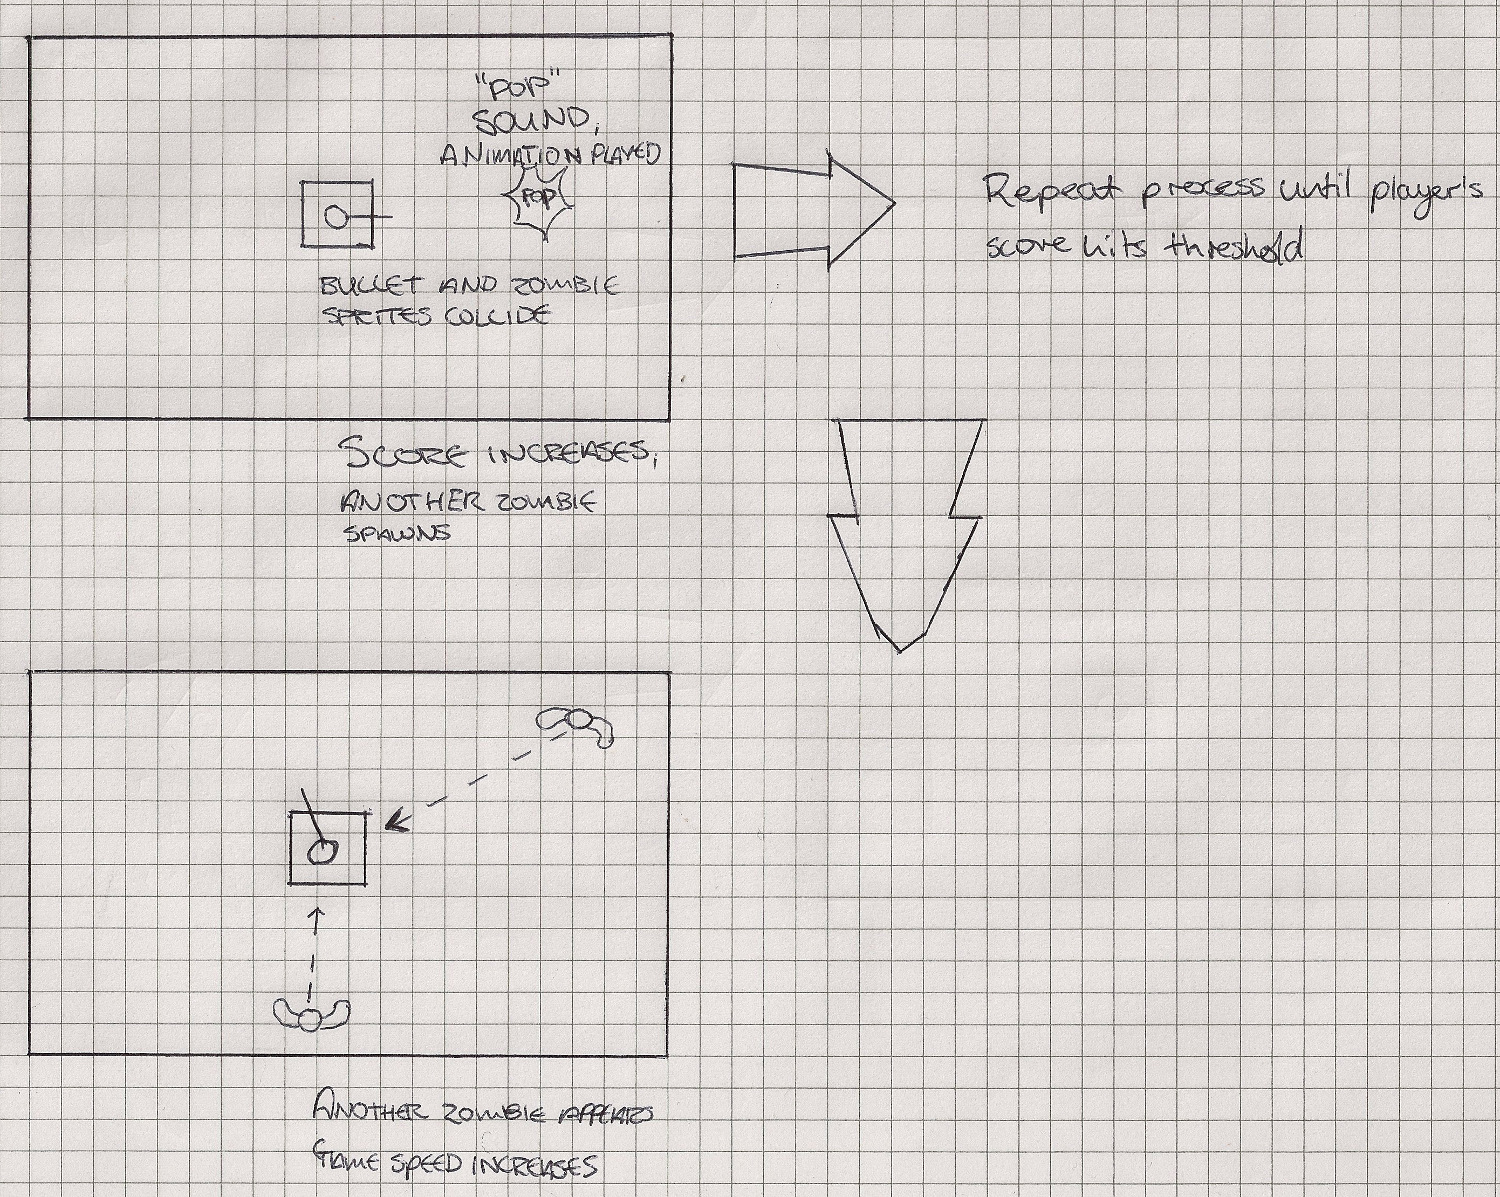
\includegraphics[height=0.7\columnwidth]{img/storyboard_2}
	    		\caption{Second storyboard in sequence}
    		\end{figure}
    		
    		\clearpage
    		\begin{figure}[htp]
	    		\vspace{1.8in}
	    		\centering
                    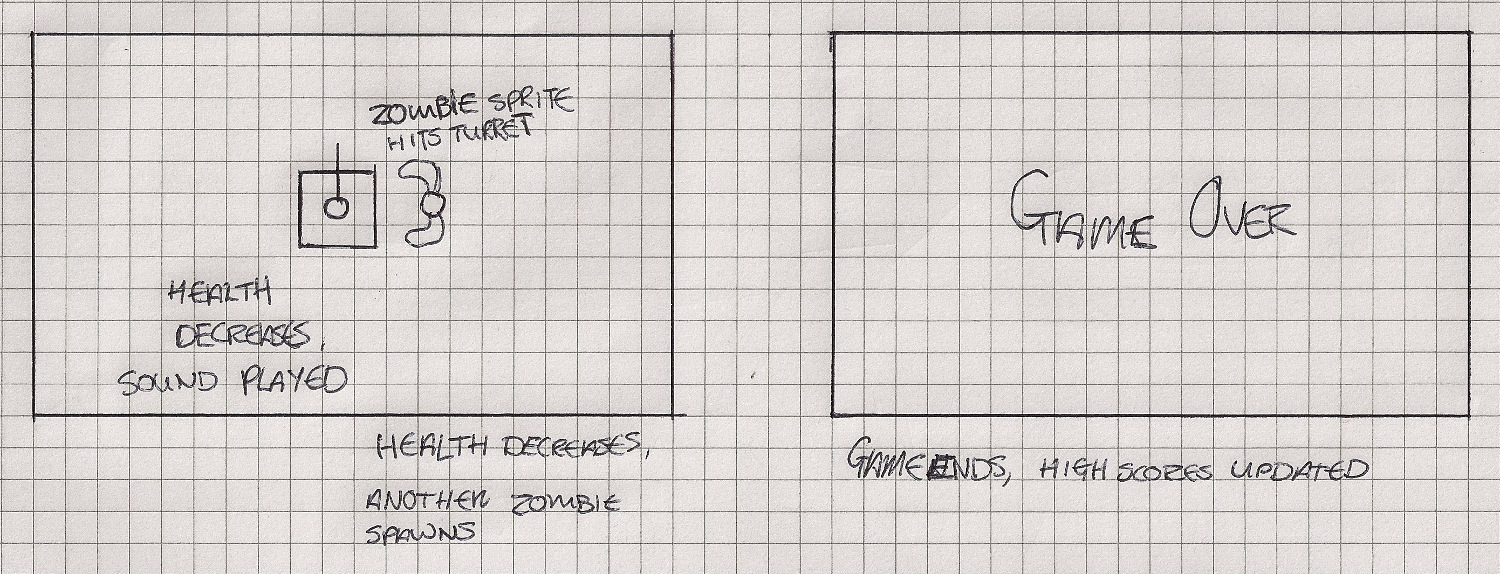
\includegraphics[width=0.8\columnwidth]{img/storyboard_3}
	    		\caption{Third storyboard in sequence}
    		\end{figure}
        \end{subsection}
    \end{section}
\end{landscape}
\end{document}

%									Other useful bits and pieces
%\begin{section}{section_name}										% Start section
%\end{section}														% End section
%\begin{center} \end{center}										% Center stuff
%\includegraphics[width=0.75\columnwidth]{example_figure}			% Insert image
%\pseudocode{filename}{caption}										% Insert highlighted code snippet
%\clearpage															% Clear page after section
%\url{http://www.google.com/}										% Include URL
%\nocite{citationName}												% Cite to bibliography but not text
%\cite{citationName}												% Include reference